% This is "sig-alternate.tex" V2.1 April 2013
% This file should be compiled with V2.5 of "sig-alternate.cls" May 2012
%
% This example file demonstrates the use of the 'sig-alternate.cls'
% V2.5 LaTeX2e document class file. It is for those submitting
% articles to ACM Conference Proceedings WHO DO NOT WISH TO
% STRICTLY ADHERE TO THE SIGS (PUBS-BOARD-ENDORSED) STYLE.
% The 'sig-alternate.cls' file will produce a similar-looking,
% albeit, 'tighter' paper resulting in, invariably, fewer pages.
%
% ----------------------------------------------------------------------------------------------------------------
% This .tex file (and associated .cls V2.5) produces:
%       1) The Permission Statement
%       2) The Conference (location) Info information
%       3) The Copyright Line with ACM data
%       4) NO page numbers
%
% as against the acm_proc_article-sp.cls file which
% DOES NOT produce 1) thru' 3) above.
%
% Using 'sig-alternate.cls' you have control, however, from within
% the source .tex file, over both the CopyrightYear
% (defaulted to 200X) and the ACM Copyright Data
% (defaulted to X-XXXXX-XX-X/XX/XX).
% e.g.
% \CopyrightYear{2007} will cause 2007 to appear in the copyright line.
% \crdata{0-12345-67-8/90/12} will cause 0-12345-67-8/90/12 to appear in the copyright line.
%
% ---------------------------------------------------------------------------------------------------------------
% This .tex source is an example which *does* use
% the .bib file (from which the .bbl file % is produced).
% REMEMBER HOWEVER: After having produced the .bbl file,
% and prior to final submission, you *NEED* to 'insert'
% your .bbl file into your source .tex file so as to provide
% ONE 'self-contained' source file.
%
% ================= IF YOU HAVE QUESTIONS =======================
% Questions regarding the SIGS styles, SIGS policies and
% procedures, Conferences etc. should be sent to
% Adrienne Griscti (griscti@acm.org)
%
% Technical questions _only_ to
% Gerald Murray (murray@hq.acm.org)
% ===============================================================
%
% For tracking purposes - this is V2.0 - May 2012

\documentclass{sig-alternate-05-2015}

\usepackage[usenames,dvipsnames]{xcolor}
\usepackage{listings}

\begin{document}

% Copyright
\setcopyright{acmcopyright}
%\setcopyright{acmlicensed}
%\setcopyright{rightsretained}
%\setcopyright{usgov}
%\setcopyright{usgovmixed}
%\setcopyright{cagov}
%\setcopyright{cagovmixed}


% DOI
%\doi{10.475/123_4}

% ISBN
%\isbn{123-4567-24-567/08/06}

%Conference
\conferenceinfo{SAICSIT '15}{September 28--30, 2015, Stellenbosch, ZAR}

%\acmPrice{\$15.00}

%
% --- Author Metadata here ---
%\conferenceinfo{WOODSTOCK}{'97 El Paso, Texas USA}
%\CopyrightYear{2007} % Allows default copyright year (20XX) to be over-ridden - IF NEED BE.
%\crdata{0-12345-67-8/90/01}  % Allows default copyright data (0-89791-88-6/97/05) to be over-ridden - IF NEED BE.
% --- End of Author Metadata ---

\title{Aspect-Oriented Parallel Programming Using AspectC++ and OpenCL}
%\subtitle{[Extended Abstract]
%\titlenote{A full version of this paper is available as
%\textit{Author's Guide to Preparing ACM SIG Proceedings Using
%\LaTeX$2_\epsilon$\ and BibTeX} at
%\texttt{www.acm.org/eaddress.htm}}}
%
% You need the command \numberofauthors to handle the 'placement
% and alignment' of the authors beneath the title.
%
% For aesthetic reasons, we recommend 'three authors at a time'
% i.e. three 'name/affiliation blocks' be placed beneath the title.
%
% NOTE: You are NOT restricted in how many 'rows' of
% "name/affiliations" may appear. We just ask that you restrict
% the number of 'columns' to three.
%
% Because of the available 'opening page real-estate'
% we ask you to refrain from putting more than six authors
% (two rows with three columns) beneath the article title.
% More than six makes the first-page appear very cluttered indeed.
%
% Use the \alignauthor commands to handle the names
% and affiliations for an 'aesthetic maximum' of six authors.
% Add names, affiliations, addresses for
% the seventh etc. author(s) as the argument for the
% \additionalauthors command.
% These 'additional authors' will be output/set for you
% without further effort on your part as the last section in
% the body of your article BEFORE References or any Appendices.

\numberofauthors{1} %  in this sample file, there are a *total*
% of EIGHT authors. SIX appear on the 'first-page' (for formatting
% reasons) and the remaining two appear in the \additionalauthors section.
%
\author{
% You can go ahead and credit any number of authors here,
% e.g. one 'row of three' or two rows (consisting of one row of three
% and a second row of one, two or three).
%
% The command \alignauthor (no curly braces needed) should
% precede each author name, affiliation/snail-mail address and
% e-mail address. Additionally, tag each line of
% affiliation/address with \affaddr, and tag the
% e-mail address with \email.
%
% 1st. author
\alignauthor
Robert Clucas\\
       \affaddr{University of the Witwatersrand}\\
       \affaddr{1 Jan Smuts Avenue}\\
	   \affaddr{Johannesburg, South Africa}\\
       \email{robert.clucas@students.wits.ac.za}
}
% There's nothing stopping you putting the seventh, eighth, etc.
% author on the opening page (as the 'third row') but we ask,
% for aesthetic reasons that you place these 'additional authors'
% in the \additional authors block, viz.
%\additionalauthors{Additional authors: John Smith (The Th{\o}rv{\"a}ld Group,
%email: {\texttt{jsmith@affiliation.org}}) and Julius P.~Kumquat
%(The Kumquat Consortium, email: {\texttt{jpkumquat@consortium.net}}).}
\date{\today}
% Just remember to make sure that the TOTAL number of authors
% is the number that will appear on the first page PLUS the
% number that will appear in the \additionalauthors section.

\maketitle
\begin{abstract}
This paper provides a sample of a \LaTeX\ document which conforms,
somewhat loosely, to the formatting guidelines for
ACM SIG Proceedings. It is an {\em alternate} style which produces
a {\em tighter-looking} paper and was designed in response to
concerns expressed, by authors, over page-budgets.
It complements the document \textit{Author's (Alternate) Guide to
Preparing ACM SIG Proceedings Using \LaTeX$2_\epsilon$\ and Bib\TeX}.
This source file has been written with the intention of being
compiled under \LaTeX$2_\epsilon$\ and BibTeX.

The developers have tried to include every imaginable sort
of ``bells and whistles", such as a subtitle, footnotes on
title, subtitle and authors, as well as in the text, and
every optional component (e.g. Acknowledgments, Additional
Authors, Appendices), not to mention examples of
equations, theorems, tables and figures.

To make best use of this sample document, run it through \LaTeX\
and BibTeX, and compare this source code with the printed
output produced by the dvi file. A compiled PDF version
is available on the web page to help you with the
`look and feel'.
\end{abstract}


%
% The code below should be generated by the tool at
% http://dl.acm.org/ccs.cfm
% Please copy and paste the code instead of the example below. 
%

\begin{CCSXML}
	<ccs2012>
	<concept>
	<concept_id>10010147.10010169.10010175</concept_id>
	<concept_desc>Computing methodologies~Parallel programming
	languages</concept_desc>
	<concept_significance>500</concept_significance>
	</concept>
	<concept>
	<concept_id>10010520.10010521.10010528</concept_id>
	<concept_desc>Computer systems organization~Parallel
	architectures</concept_desc>
	<concept_significance>300</concept_significance>
	</concept>
	<concept>
	<concept_id>10011007.10011006.10011050</concept_id>
	<concept_desc>Software and its engineering~Context specific
	languages</concept_desc>
	<concept_significance>300</concept_significance>
	</concept>
	</ccs2012>
\end{CCSXML}

\ccsdesc[500]{Computing methodologies~Parallel programming languages}
\ccsdesc[300]{Computer systems organization~Parallel architectures}
\ccsdesc[300]{Software and its engineering~Context specific languages}
%
% End generated code
%

%
%  Use this command to print the description
%
\printccsdesc

% We no longer use \terms command
%\terms{Theory}

\keywords{Aspect; device; host; pointcut; advice}

\section{Introduction}\label{sec:intro}
In recent years parallel systems become more established as processor core
frequencies began to plateau. The result of this was parallel systems which made
use multiple core CPUs and many core GPUs. The cores used for CPUs and GPUs differ 
in complexity and are hence advantageous for different tasks. GPUs use many 
(up to thousands), simple cores to increase computational efficiency, while CPUs 
use fewer, complex cores which generally have higher frequencies. Due to the
number of cores available when using a GPU, GPUs are suited to data parallel
tasks where the same operation can be performed on each element of a high
dimensional dataset. Modern CPUs can also provide data parallelism through
single instruction multiple data(SIMD) operations, however, due to having fewer
cores they provide lower levels of performance increase and require large
amounts of power to perform the instruction level parallelism \cite{kumar:power}.
General-Purpose GPU (GPGPU) programming involves combining CPU's and GPU's 
into a single, hybrid system which provides increased computational performance 
by using the CPU \textit{host} to pass data to the GPU \textit{device} which 
performs the computation on the data in a parallel manner.
For GPGPU programming there are two main API's available to the programmer, 
namely OpenCL \cite{opencl} and CUDA \cite{cuda}. 

OpenCL is an attempt to provide a standard API for programming parallel capable
hardware. It provides support for all main CPU and GPU hardware vendors, namely 
Nvidia, AMD and Intel. This wide range of support is advantageous as a 
parallel implementation using the OpenCL API could run on both the CPU and GPU
present in the hybrid system, simultaneously. CUDA applies a similar methodology 
and also provides and API for writing programs which can be executed on parallel capable
hardware, however, it is specific to Nvidia hardware and hence parallel kernels
cannot be executed on CPUs or GPUs from any other hardware vendor.

These parallel systems are more difficult to 
program when compared to traditional, sequential systems. To perform parallel
computation on the \textit{device} using OpenCL the generalised sequence of
events, which is similar to the generalised sequences of events for a CUDA C
program \cite{cudaseq}, is (The colors after the description relate to the
example given in Listing~\ref{vectcl})
\begin{enumerate}
	\item{Initialize the \textit{host} data (Green)}
	\item{Setup OpenCL variables, which involves (Red):
			\begin{itemize}
				\item{Setting the OpenCl platform }
				\item{Creating the OpenCL Context }
				\item{Setting the parallel device to use }
				\item{Creating the OpenCL command queue }
		\end{itemize} }
	\item{Creating the OpenCL kernel (Blue)}
	\item{Create OpenCL buffers to move data from \textit{host} to
		\textit{device}(Magenta)}
	\item{Execute kernel on parallel device (Green)}
	\item{Move results back from \textit{device} to \textit{host} (Magenta)}
\end{enumerate}
which is a lengthy sequence of events to perform parallel computation.
Comparatively, to do the same computation using only the \textit{host}, only two
steps would be required, steps 3 and 5 defined above. All other steps increase
the complexity of performing parallel programming and cross-cut the intention of
the core code (code directly related to the problem) which is the execution of
the operations on the data. This is illustrated by a comparison of
Listings~\ref{vectcpp} and \ref{vectcl} which show a vector addition kernel
implementation using C++ and OpenCL respectively.

\lstset{language		= c++,
		frame			= single,
		tabsize			= 2,
		breaklines		= true,
		basicstyle		= \scriptsize ,
		escapeinside	= {<@}{@>},
		captionpos		= b
	}

\begin{lstlisting}[caption=Vector addition using
C++,label=vectcppi,float=[t!]]
#define T float
void VectAdditionC++(int argc, char** argv) {
	<@\color{Green!85}{// Instantiate vector add class}@>
	VectAddCppClass vectAdd;
	<@\textcolor{Green!85}{// Declare data vectors}@>
	vector<T>  in1, in2, out;
	<@\textcolor{Green!85}{// Fill data vectors}@>
	for (int i = 0; i < NUM_ELEMENTS; i++) {
		out.push_back(0.f);
		in1.push_back(rand());
		in2.push_back(rand());
	}
	<@\textcolor{Green!85}{// Execute Kernel}@>
	vectAdd.RunKernel(in1, in2, out);
}
\end{lstlisting}


The need for GPGPU programming arises from the computational complexity of the
algorithms which results in non-GPGPU systems not being able to compute the
algorithm in sufficient time. The additional complexities make parallel
development inefficient and require programmers to learn the complex OpenCL and
CUDA API's, hence programmers are generally reluctant to take on the learning
curve required for parallel programming. However, the computational speed up
provided by GPGPU programming is still required and thus the complex, low-level
interaction between the \textit{host} and \textit{device} must be overcome to
gain access to the increased computational performance.

To remove the requirement of the programmer to deal with this complexity, 
aspect-oriented programming  (AOP) \cite{gregor:aop} can provide a solution which 
allows the cross-cutting components to be \textit{woven} into the core computational 
code at compile time, but being modularised into aspects before compile time, resulting 
in simple core code which consists only of code directly related to the program
intention, and aspects which contain the code which cross-cuts the program's
intention.

Aspects are a relatively new concept in computer science and work on aspects on
C++ is limited. An AOP implementation for C++ has been available since 2005 in
the form of AspectC++ \cite{acpp}. Furthermore the use of aspects in low-level
parallel programming is even more limited, however, numerous proposals have been
provided which aim to reduce the complexities of low-level parallel programming
(summarised in Section~\ref{sec:related}). This paper presents the Aspect Parallel
Programming \textit{APP} model which makes use of aspects, using AspectC++, to 
hide the above mentioned complexities present in parallel programming using
OpenCL, from the programmer. 

The aspects perform both the static components - the initialisation of the
OpenCL variables - and the dynamic components - creating the relevant buffers
and allocating and deallocating memory on the host and device when kernels are
executed. The kernel function is not dealt with by the \textit{APP} model. This
choice was made since the kernel is specific to the implementation of the
algorithm and should thus be given to the developer. Converting C++ code to an
OpenCL kernel would require building a compiler, which is not the aim of the
proposal, or performing runtime conversion, which would result in performance
loss. To write a kernel the developer does not need to learn the OpenCL API, but
only needs an understanding of how parallel computation it performed in terms of
the thread arrangement, which should be known if the programmer would like to
parallelize their algorithm. 

The \textit{APP} model has two main goals:
\begin{itemize}
	\item{To allow for a parallel implementation 
			which is comparatively simple, in terms of code structure and number
			of line, with a sequential, C++ only implementation 
			but that also allows direct access to the low-level hardware
			through aspects - if required by the programmer
		}
	\item{Provides performance which is comparable with a non-aspect
			implementation written using OpenCL or CUDA
		}
\end{itemize}

\begin{lstlisting}[caption=Vector addition using
OpenCL highlighting the different cross-cutting components,label=vectcl,float=[t!]]
#define T float
void VectAdditionCl(int argc, char** argv) {
	<@\color{Red!85}{// Declare OpenCl variables}@>
	vector<cl::Platform> platforms;
	vector<cl::Device>   devices;
	vector<cl:Buffer>    buffers;
	cl::Context          context;
	cl::CommandQueue     queue;
	cl::Program          program;
	cl::Kernel           kernel;
	<@\textcolor{Green!85}{// Declare data vectors}@>
	vector<vector<T>>    inputs;
	vector<T>  in1, in2, out;
	<@\textcolor{Green!85}{// Fill data vectors}@>
	for (int i = 0; i < NUM_ELEMENTS; i++) {
		out.push_back(0.f);
		in1.push_back(rand());
		in2.push_back(rand());
	}
	inputs.push_back(in1); inputs.push_back(in2);
	<@\color{Red!85}{// Get OpenCL Platforms}@>
	clPlatform::get(&platforms);
	<@\color{Red!85}{// Create context params}@>
	cl_context_properties cps[3] = {
		CL_CONTEXT_PLATFORM,
		(cl_context_properties)(platforms[0])(),
		0 
	};
	<@\color{Red!85}{// Create OpenCL context}@>
	context = cl::Context(CL_DEVICE_TYPE_GPU, cps);
	<@\color{Red!85}{// Get available devices}@>
	devices = context.getInfo<CL_CONTEXT_DEVICES>();
	<@\color{Red!85}{// Create command queue}@>
	queue = cl::CommandQueue(context, devices[0]);
	<@\textcolor{Blue!85}{// Get kernel source}@>
	ifstream kSource("vectadd.cl");
	<@\textcolor{Blue!85}{// Convert kernel source to string}@>
	string kstring(
		istreambuf_iterator<char>(kSource),
		(istream_buf_iterator<char>()) );
	<@\textcolor{Blue!85}{// Create OpenCL program source}@>
	cl::Program::Sources source(1, 
		make_pair(kstring.c_str(), 
		          kstring.length() + 1) );
	<@\textcolor{Blue!85}{// Create OpenCL program}@>
	program = cl::Program(context, source);
	<@\textcolor{Blue!85}{// Create OpenCL kernel}@>
	kernel = cl::Kernel(program, "vectadd");
	<@\textcolor{Magenta!85}{// Create input buffers}@>
	for (auto& input : inputs) {
		buffers.emplace_back(context, 
			CL_MEM_READ_ONLY, 
			input.size() * sizeof(T) );
		queue.enqueueWriteBuffer(buffers.back(),
			CL_TRUE, 0, input.size() * sizeof(T),
            &input[0] );
	};
	<@\textcolor{Magenta!85}{// Create output buffer}@>
	buffers.emplace_back(context, CL_MEM_WRITE_ONLY,
		out.size() * sizeof(T) );
		<@\textcolor{Magenta!85}{// Set kernel arguments}@>
	for (int i = 0; i < buffers.size(); i++) {
		kernel.setArg(i, buffers[i]);
	}
	<@\textcolor{Magenta!85}{// Set thread dimensions}@>
	cl::NDRange global(inputs[0].size());
	cl::NDRange local(1);
	<@\textcolor{Green!85}{// Execute Kernel}@>
	queue.enqueueNDRangeKernel(kernel,
		cl::NullRange, global, local);
	<@\textcolor{Magenta!85}{// Get results from GPU}@>
	T* res[NUM_ELEMENTS];
	queue.enqueueReadBuffer(buffers.back(),
		CL_TRUE, 0, out.size() * sizeof(T), res);
}
\end{lstlisting}
The rest of the report is structured as follows: Section~\ref{sec:related}
reviews work related to the simplification of parallel programming both using
aspects and other methods;
Section~\ref{sec:aspects} describes the \textit{APP} programming model and the use 
of AspectC++, and its features, to achieve the above mentioned goals; Section~\ref{sec:results}
presents the results of implementations of \textit{APP} to two problem domains,
SAXPY and Black Scholes option pricing;
Section~\ref{sec:evaluation} provides a comparison of the \textit{APP} model 
with both a non-aspect non-parallel C++ solution, and a
non-aspect parallel OpenCL solution, in terms of both performance and code
complexity and comments on the limitations of the \textit{APP} model; 
Section~\ref{sec:conclusion} concludes and Section~\ref{sec:future}
discusses directions of exploration for future work in this area.

\section{Related Work}\label{sec:related}

With the increasing popularity and necessity of parallel implementations,
attempts to minimise the complexity of writing parallel code have both increased
in number and made the task simpler. OpenCL and Nvidia CUDA are both examples of
this. They provide extensions to the C language and provide low-level
access to the parallel hardware. As mentioned in Section~\ref{sec:intro} this
introduces cross-cutting code that `tangles' the core code. Furthermore, while
access is given to the parallel capable hardware, the API's are extensive and
have steep learning curves.

APIs, frameworks, and entirely separate languages, which hide the low-level 
interactions with the parallel capable hardware from the programmer, have been
proposed. These systems provide wrappers around the low-level interfaces 
which often reduces performance, a key consideration in parallel programming,  
and requires the programmer to learn an additional set of API functions.

CuPP \cite{breit:cupp} provides a C++ framework designed to increase the ease of implementing parallel
applications using CUDA. It provides both low-level and high-level interfaces
which interact with the parallel capable hardware, hence providing a C++
interface for programming parallel applications. This is also an attempt to wrap
the cross-cutting code into modules such that it is hidden from  the programmer,
but in an object oriented manner thus resulting in more code than what is
required for a traditional CUDA implementation. Since the framework is built
around CUDA, support is only provided for Nvidia devices.

CAF \cite{schmidt:actor} \cite{schmidt:actor1} uses the actor model to allow
computation to be performed in a distributed manner. It provides bindings for
OpenCL which allow the programmer to specify only the OpenCL kernel from which
CAF creates an actor capable of executing the kernel. The framework allows
computation on a vast number of parallel capable devices, which is a notable
feature. However, providing support for so many devices introduces overhead and makes 
the framework very large. Furthermore it requires learning the actor model 
which introduces complexity into learning the parallel programming process.

C++ AMP \cite{microsoft:amp} provides extensions to the C++ language which allow 
data parallel capable hardware to be used to accelerate computation. C++ AMP is 
only available for the Windows environment and is thus limited in scope which is
contrary to the generality the proposed aspect implementation aims to provide.

RapidMind \cite{rapidmind} and Brook \cite{brook}, while are similar to standard
C++, essentially define new languages which allow for parallel acceleration.

RapidMind provides a parallel programming environment which, by
taking advantage of C++ template metaprogramming, provides the programmer 
with three data types: \textit{Value}, \textit{Array}, and \textit{Program}.
The \textit{Value} and \textit{Array} data types hold data elements and and
groups of data elements, respectively. The \textit{Program} data type stores
operations which can act on \textit{Array} data types in a parallel manner.
The \textit{Program} data type is essentially same concept as the kernel provided 
by Nvidia and OpenCL, in the C++ language. RapidMind also makes use of macros,
which add complexity to the code, rather simplifying the code - the intention of
aspects.

Brook provides high-level abstractions to hide the low-level parallel
programming complexities from the programmer. Similarly to RapidMind there 
are three abstractions which create the high-level parallel programming 
environment: \textit{Stream}, \textit{Kernel}, and \textit{Reduction}. The 
\textit{Stream} deals with the data, while the \textit{Kernel}, similar to both 
the kernel in the Nvidia and OpenCL models and the \textit{Program} data type for 
RapidMind, allow operations to be defined which act on the \textit{Streams} (data). 
The \textit{Reduction} is provided to generate a result from a high dimensional 
\textit{stream}.

Both RapidMind and Brook do a lot of work at runtime to allow computation to be
execution on the device, as well as to move the data to the device memory. This
reduces their performance when compared to CUDA or OpenCL implementations, which
has resulted in these parallel environments not gaining high levels of acceptance 
within the parallel development community.

Work done on the use of aspects for parallel programming is limited, especially
for low-level programming which interfaces directly with the parallel hardware.
Use for aspects in a parallel context is proposed by \cite{jaspect},
however, Java is used and the model is based on multi-core CPUs and does not include the
numerous complexities which arise from having other computational devices such
as GPUs.

A new, parallel aspect language, based on AspectC++, is proposed by
\cite{aopstream}. Features closely related to AspectC++, but more specific to
parallel programming. are defined to hide most of the complexities from the
programmer. The result is a large  reduction of the cross-cutting components
present in low-level parallel programming. The system allows the core computations 
to be defined using C++. The aspect model defines a \textit{kernel} feature
which behaves in the same way as \textit{advice} in AOP. Furthermore the memory
structure of the device is encapsulated using templates and allows the
programmer to specify the type of \textit{device} memory to be used in C++. A
compiler is used to weave the defined language into the C++ core code. The
performance reduction of only $\approx$20$\%$ was achieved. The aspect model is
not yet fully functional and is specific to parallel programming, thus at this
stage could not be used to modularize non-parallel cross-cutting concerns into
aspects.

The \textit{APP} model provides a few advantages over the related work:
(1) The aspect components use AspectC++ which is based on standard
C++ and allows the core code to be written in standard C++ rather than providing
an alternative language for parallel programming. This is beneficial for large
systems as cross-cutting concerns arising from non-parallel complexities can be
modularised using AspectC++. (2) Low-level parallel programming complexities are 
hidden from the programmer by the aspects. This results in code code the has no
components which cross-cut the code's intention, and thus kernel functions which
can be executed from the \textit{host} with a single function call of an
instantiated C++ class. (3) There is negligible loss in performance. This is because 
AspectC++ weaves the aspects into the core code before compilation so that to
the compiler the code looks like the tangled code, but to the programmer is
`untangled'.

\section{The Aspect-Oriented Parallel \\ Programming (APP) Model}\label{sec:aspects}

The \textit{APP} model presented in this section allows the programmer to
write parallel programs in traditional C++ with the addition of the kernel
function which performs tasks on some data in a parallel manner. The aspects
components are written using AspectC++ and provide the functionality of the
cross-cutting OpenCL code, hence `untangling' the core code. To demonstrate the
use of the \textit{APP} model, the OpenCL vector addition of
Listing~\ref{vectcl} will be used as an example. 

\subsection{Abstract ClContext Aspect}

AspectC++ is based on C++ and hence provides functionality for both inheritance
and polymorphism. The \textit{APP} model makes use of these features and defines
an abstract aspect, the \textit{ClContext} aspect, which provides the core C++ code with 
the cross-cutting OpenCL components necessary for executing a parallel kernel.
The OpenCL  components, both variables and member functions, are defined in the abstract 
aspect and are inherited by the derived aspect. Any additional OpenCL
functionality, which may improve specific parallel implementations, can then be 
defined in the derived aspect if required. Polymorphism is provided by AspectC++ 
through virtual pointcuts. Virtual pointcuts were used by the abstract
\textit{ClContext} aspect to define an interface which allows the derived aspect
to specify which C++ core classes require parallel capability.
The \textit{CoreClasses} pointcut in Listing~\ref{slice} shows this. This allows
the abstract aspect to provide any general functionality which should be present
for a parallel class, without defining which class the aspect should weave the
functionality into. Listing~\ref{dslice} shows the derived aspect, which uses
the virtual \textit{CoreClasses} to define which of the C++ core classes the
OpenCL functionality should be woven into.

\subsection{OpenCL Variable Introduction}

Observing Listing~\ref{vectcl} there numerous OpenCL specific variables
(variables defined below the red comments) which are required to setup the 
OpenCL environment so that the kernel can be executed on the parallel capable 
hardware. Many of these variables are required to be modified or recreated each
time a new kernel needs to be executed, requiring a significant amount of 
overhead when compared to the C++ version of Listing~\ref{vectcpp}.

AspectC++ provides the \textit{slice} feature for defining C++ classes within
aspects. Furthermore, it allows for \textit{advice} to be defined for the
the virtual pointcut and this advice can use C++ inheritance to weave the
\textit{slice} class as a base class for C++ core classes, or to derive from 
C++ core classes. Using these features, the \textit{APP} model defines the 
\textit{ClInstance} \textit{slice} class within the abstract \textit{ClContext} class.  
The \textit{CLInstance} class has the cross-cutting OpenCL variables as public
variables, and the cross-cutting OpenCL operations as private member functions. 
The advice for the virtual pointcut tells the aspect weaver to weave the
\textit{slice} class as a base class of the C++ core class requiring parallel
capability. 
Listing~\ref{slice} shows the \textit{slice} class within the abstract aspect,
as well as the cross-cutting variables (below the red comments as per 
Listing~\ref{vectcl}) and member functions which provide the cross-cutting
OpenCL setup.

\begin{lstlisting}[caption=Abstract aspect which defined the OpenCL variables
required for parallel programming,label=slice,float=[!t]]
// ClContext.ah
aspect ClContext {
	class ClInstance {
	public:
		<@\color{Red!85}{// OpenCL variables}@>
		vector<cl::Platform> platforms;
		vector<cl::Device>   devices;
		vector<cl::Buffer>   buffers
		cl::clContext        context;
		cl::CommandQueue     queue;
		cl::Kernel           kernel;
		cl::Program          program;
		// Other variables and functions 
	private:
		<@\color{Red!85}{// Setup OpenCL variables}@>
		void SetupOpenCl(string devType, string kSource);
		<@\color{Blue!85}{// Setup OpenCL kernel}@>
		void SetupKernel(string kSource, string kName);
		<@\color{Magenta!85}{// Manage buffers on kernel execution}@>
		void ManageBuffers(vector<vector<T>>* inputs,
		                   vector<vector<T>>* outputs);
	};
	// Interface for defining C++ core classes
	pointcut virtual CoreClasses() = 0;

	// Specify ClInstance as baseclass of classes
	// defined by CoreClasses()
	advice CoreClasses() : baseclass(ClInstance);

  // Other aspect components
};
\end{lstlisting}

\begin{lstlisting}[caption=Derived aspect defining the core classes which need
the OpenCL variables,label=dslice,float=[!t]]
#include ``ClContext.ah"
aspect VectAdd : ClContext {
	// Define C++ core class to weave OpenCL 
	// functionality into
	pointcut CoreClasses() = "ParVectAddCppCore";
};
\end{lstlisting}

\subsection{OpenCL Setup Function Introduction}

Again observing Listing~\ref{vectcl}, a large amount of the cross-cutting code
comes from the operations on the OpenCL variables. These operations (below the
red comments in the Listings) are for the setup of the OpenCL environment and 
determine the available devices and platforms, create the OpenCL context. They
cross-cut the C++ core code since they are not related to the intention of the
program. Furthermore, these operations are generic - they are the same for any 
OpenCL program - they can be defined performed in functions of the \textit{ClInstance} 
\textit{slice} class. The operations for creating the kernel (below the blue 
comments in Listings) have the same problems and hence can also be performed 
in functions of th \textit{ClInstance} \textit{slice} class. 

The \textit{ClContext} aspect then defines a \textit{ClSetup} pointcut to
specify where in the C++ core code these functions should be executed on
construction of the C++ core class. To provide the programmer with flexibility 
when writing the C++ core class teh \textit{ClSetup} advice makes use of the
\textit{tjp} pointer AspectC++ provides. The \textit{tjp} pointer provides the
aspect with access to the C++ core class into which the aspect will be woven.
Using \textit{tjp->that()} in an aspect is equivalent to using \textit{this}
within the C++ core class. This feature was used to allow the programmer to
specify the computation device (CPU or GPU) and the kernel source file and name
as variables of the C++ core class. Using AcpectC++'s \textit{tjp->that()}
the aspect can use the values provided by the programmer from the C++ core code
to setup the OpenCL environment as required. 
Listing~\ref{clsetup} shows the definition of \textit{ClSetup} pointcut and its 
advice which calls the private member functions of the \textit{ClInstance} class 
as defined in Listing~\ref{slice}.

\begin{lstlisting}[caption=Abstract aspect with the pointcut and advice for
OpenCL setup,label=clsetup,float=[!t]]
// ClContext.ah
aspect ClContext {
	class ClInstance {
		// As per Listing 3 ...
	};
	// Other pointcuts and advice

	// Pointcut which defines where the OpenCL
	// setup function should be woven
	pointcut ClSetup = construction(CoreClasses());
  
	// Advice specifying how the OpenCL
	// setup functions should be woven
	advice ClSetup() : around() {
		<@\color{Red!85}{// Setup OpenCL variables}@>
		tjp->that()->SetupOpenCl(
			tjp->that()->devType, tjp->that()->kSource);
		<@\color{Blue!85}{// Setup OpenCL kernel}@>
		tjp->that()->SetupKernel(
			tjp->that()->kSource, tjp->that()->kName); 
		// Continue with core class constructor
		tjp->proceed();
	}
};
\end{lstlisting}

\subsection{RunKernel Interface}

Executing the kernel is the main component of a parallel application. Before the
kernel is run the data on which the kernel operates must be moved from the
memory of the \textit{host} to the memory of the \textit{device}. Once the
kernel has finished executing, the results reside in the memory of the
\textit{device} and are not available to the \textit{host} until transferred
back from the \textit{device} memory to the \textit{host} memory. This is done
using the cl::Buffer type in OpenCL. These operations are shown in Listing~\ref{vectcl} 
below the magenta comments. This process of memory allocation, movement, and
deallocation is not required for a C++ implementation, thus cross-cut's the
program's main intention. Furthermore, memory management is a difficult problem
in the C and C++ language, which is exaggerated by the introduction of device
memory.  These operations are required each time the kernel is executed and
result in the amount of cross-cutting code growing linearly with the number of
kernels and kernel calls. 

These problems are solved through aspects by defining a virtual,
\textit{RunKernel}, function in the \textit{ClInstance} \textit{slice} class. 
The \textit{runKernel} function provides an interface for the programmer in 
the C++ core class. Since the \textit{ClInstance} \textit{slice} class is a 
baseclass of any C++ core class requiring parallel functionality, the
\textit{RunKernl} must be defined in the C++ core class and hence will always be
present. By defining the \textit{RunKernel} function as an interface the
\textit{ClContext} aspect can define advice to implement the cross-cutting code
each time the C++ core class calls the \textit{RunKernel} function.

The \textit{RunKernel} function specifies that the arguments provided from the
C++ code code must be vectors which hold the input and output data for the
kernel, which are the input and output variables for the computation. This
allows the C++ core code to execute a kernel by simply calling the
\textit{RunKernel} function and passing the inputs and outputs as function
arguments, as shown by Listing~\ref{crunkernl} The \textit{tjp} pointer is 
again used, but this time to access the \textit{RunKernel} function arguments 
and hence the input and output data for the kernel so that the buffers can be managed.

Listing~\ref{runkernel} shows the \textit{ManageKernel} pointcut and advice
which calls the \textit{ManageBuffers} function in the \textit{CLInstance} class
to perform the cross-cutting memory management between the \textit{host} and
\textit{device}

\begin{lstlisting}[caption=Abstract aspect components with hide kernel
cross-cutting concerns,label=runkernel,float=[!t]]
// ClContext.ah
#define T float
aspect CLContext {
	class ClInstance {
	public:
		<@\color{Red!85}{// OpenCL variables ...}@>
		<@\color{Green!85}{// Execute kernel}@>
		virtual void RunKernel(
			vector<vector<T>>& inputs,
			vector<vector<T>>& outputs) = 0;
	private:
		<@\color{Red!85}{// Setup OpenCL variables ...}@>
		<@\color{Blue!85}{// Setup OpenCL kernel ...}@>
		<@\color{Magenta!85}{// Manage memory buffers}@>
		void ManageBuffers(
			vector<vector<T>>* inputs,
			vector<vector<T>>* outptus);
	};
	// Other advice and pointcuts 

	// Pointcut defines where the memory 
	// buffers should be managed
	pointcut ManageKernel() = 
		execution("% ...::...::RunKernel(...)") &&
		within(CoreClasses());

	// Advice specifies how to manage buffers
	advice ManageKernel() : before() {
		<@\color{Magenta!85}{// Manage memory buffers}@>
		tjp->that()->ManageBuffers(tjp->arg<0>(),
								   tjp->arg<1>());
  }
};
\end{lstlisting}

\begin{lstlisting}[caption=C++ core class executing a pallel kernel using
standard c++,label=crunkernel,float=[!t]]
#define T float
int VectAddCpp(int argc, char** argv) {
	<@\color{Green!85}{// Instantiate vect addition class }@>
	ParVectAddCppCore vectAdd;
	<@\color{Green!85}{// Create input and output buffers}@>
	vector<vector<T>> inputs;
	vector<vector<T>> outputs;
	<@\color{Green!85}{// Fill vectors with data ...}@>
  
	<@\color{Green!85}{// Execute kernel}@>
	vectAdd.RunKernel(inputs, outputs);
}
\end{lstlisting}

\section{Results}\label{sec:results}

This section presents the results of application of \textit{APP} model to two
GPGPU programming problems. The first problem is essentially the `hello world`
of parallel programming and is known as SAXPY (Single-precision A*X + Y). The
second example is that of ... which is more complex and shows the use of the
\textit{APP} model to more `tangled' core code. The result are analysed in terms
of both performance and code complexity by terms of the number of lines and
modularity of the resulting code.

\subsection{SAXPY Problem}

The problem was implemented using the \textit{APP} model, OpenCL, and C++.
Various vector sizes were tested to validate that the solution using the
\textit{APP} implementation scales similarly to the OpenCL implementation.
Table~\ref{fig:saxpy} shows the performance results for SAXPY problem.

The number of lines of code for the file types for the different implementations
are given in Table~\ref{tab:saxpy}

\begin{table}[!b]
\centering
\caption{Comparison of the number of lines of code per file type for the SAXPY
problem }
\label{tab:saxpy}
\begin{tabular}{|c|c|c|c|} 
	\hline
				& APP	& OpenCL	& C++	\\ \hline
.h				&		&			&		\\ \hline
.cpp			&		&			&		\\ \hline
.ah				&		&			&		\\ \hline
.cc				&		&			&		\\ \hline
.cl				&		&			&		\\ \hline
\textbf{Total}	&		&			&		\\ \hline		
	\hline
\end{tabular}
\end{table}

\section{Evaluation and Limitations}\label{sec:evaluation}
\section{Conclusion}\label{sec:conclusion}
\section{Future Work}\label{future}

The \textit{proceedings} are the records of a conference.
ACM seeks to give these conference by-products a uniform,
high-quality appearance.  To do this, ACM has some rigid
requirements for the format of the proceedings documents: there
is a specified format (balanced  double columns), a specified
set of fonts (Arial or Helvetica and Times Roman) in
certain specified sizes (for instance, 9 point for body copy),
a specified live area (18 $\times$ 23.5 cm [7" $\times$ 9.25"]) centered on
the page, specified size of margins (1.9 cm [0.75"]) top, (2.54 cm [1"]) bottom
and (1.9 cm [.75"]) left and right; specified column width
(8.45 cm [3.33"]) and gutter size (.83 cm [.33"]).

The good news is, with only a handful of manual
settings\footnote{Two of these, the {\texttt{\char'134 numberofauthors}}
and {\texttt{\char'134 alignauthor}} commands, you have
already used; another, {\texttt{\char'134 balancecolumns}}, will
be used in your very last run of \LaTeX\ to ensure
balanced column heights on the last page.}, the \LaTeX\ document
class file handles all of this for you.

The remainder of this document is concerned with showing, in
the context of an ``actual'' document, the \LaTeX\ commands
specifically available for denoting the structure of a
proceedings paper, rather than with giving rigorous descriptions
or explanations of such commands.

\section{The {\secit Body} of The Paper}
Typically, the body of a paper is organized
into a hierarchical structure, with numbered or unnumbered
headings for sections, subsections, sub-subsections, and even
smaller sections.  The command \texttt{{\char'134}section} that
precedes this paragraph is part of such a
hierarchy.\footnote{This is the second footnote.  It
starts a series of three footnotes that add nothing
informational, but just give an idea of how footnotes work
and look. It is a wordy one, just so you see
how a longish one plays out.} \LaTeX\ handles the numbering
and placement of these headings for you, when you use
the appropriate heading commands around the titles
of the headings.  If you want a sub-subsection or
smaller part to be unnumbered in your output, simply append an
asterisk to the command name.  Examples of both
numbered and unnumbered headings will appear throughout the
balance of this sample document.

Because the entire article is contained in
the \textbf{document} environment, you can indicate the
start of a new paragraph with a blank line in your
input file; that is why this sentence forms a separate paragraph.

\subsection{Type Changes and {\subsecit Special} Characters}
We have already seen several typeface changes in this sample.  You
can indicate italicized words or phrases in your text with
the command \texttt{{\char'134}textit}; emboldening with the
command \texttt{{\char'134}textbf}
and typewriter-style (for instance, for computer code) with
\texttt{{\char'134}texttt}.  But remember, you do not
have to indicate typestyle changes when such changes are
part of the \textit{structural} elements of your
article; for instance, the heading of this subsection will
be in a sans serif\footnote{A third footnote, here.
Let's make this a rather short one to
see how it looks.} typeface, but that is handled by the
document class file. Take care with the use
of\footnote{A fourth, and last, footnote.}
the curly braces in typeface changes; they mark
the beginning and end of
the text that is to be in the different typeface.

You can use whatever symbols, accented characters, or
non-English characters you need anywhere in your document;
you can find a complete list of what is
available in the \textit{\LaTeX\
User's Guide}\cite{Lamport:LaTeX}.

\subsection{Math Equations}
You may want to display math equations in three distinct styles:
inline, numbered or non-numbered display.  Each of
the three are discussed in the next sections.

\subsubsection{Inline (In-text) Equations}
A formula that appears in the running text is called an
inline or in-text formula.  It is produced by the
\textbf{math} environment, which can be
invoked with the usual \texttt{{\char'134}begin. . .{\char'134}end}
construction or with the short form \texttt{\$. . .\$}. You
can use any of the symbols and structures,
from $\alpha$ to $\omega$, available in
\LaTeX\cite{Lamport:LaTeX}; this section will simply show a
few examples of in-text equations in context. Notice how
this equation: \begin{math}\lim_{n\rightarrow \infty}x=0\end{math},
set here in in-line math style, looks slightly different when
set in display style.  (See next section).

\subsubsection{Display Equations}
A numbered display equation -- one set off by vertical space
from the text and centered horizontally -- is produced
by the \textbf{equation} environment. An unnumbered display
equation is produced by the \textbf{displaymath} environment.

Again, in either environment, you can use any of the symbols
and structures available in \LaTeX; this section will just
give a couple of examples of display equations in context.
First, consider the equation, shown as an inline equation above:
\begin{equation}\lim_{n\rightarrow \infty}x=0\end{equation}
Notice how it is formatted somewhat differently in
the \textbf{displaymath}
environment.  Now, we'll enter an unnumbered equation:
\begin{displaymath}\sum_{i=0}^{\infty} x + 1\end{displaymath}
and follow it with another numbered equation:
\begin{equation}\sum_{i=0}^{\infty}x_i=\int_{0}^{\pi+2} f\end{equation}
just to demonstrate \LaTeX's able handling of numbering.

\subsection{Citations}
Citations to articles \cite{bowman:reasoning,
clark:pct, braams:babel, herlihy:methodology},
conference proceedings \cite{clark:pct} or
books \cite{salas:calculus, Lamport:LaTeX} listed
in the Bibliography section of your
article will occur throughout the text of your article.
You should use BibTeX to automatically produce this bibliography;
you simply need to insert one of several citation commands with
a key of the item cited in the proper location in
the \texttt{.tex} file \cite{Lamport:LaTeX}.
The key is a short reference you invent to uniquely
identify each work; in this sample document, the key is
the first author's surname and a
word from the title.  This identifying key is included
with each item in the \texttt{.bib} file for your article.

The details of the construction of the \texttt{.bib} file
are beyond the scope of this sample document, but more
information can be found in the \textit{Author's Guide},
and exhaustive details in the \textit{\LaTeX\ User's
Guide}\cite{Lamport:LaTeX}.

This article shows only the plainest form
of the citation command, using \texttt{{\char'134}cite}.
This is what is stipulated in the SIGS style specifications.
No other citation format is endorsed or supported.

\subsection{Tables}
Because tables cannot be split across pages, the best
placement for them is typically the top of the page
nearest their initial cite.  To
ensure this proper ``floating'' placement of tables, use the
environment \textbf{table} to enclose the table's contents and
the table caption.  The contents of the table itself must go
in the \textbf{tabular} environment, to
be aligned properly in rows and columns, with the desired
horizontal and vertical rules.  Again, detailed instructions
on \textbf{tabular} material
is found in the \textit{\LaTeX\ User's Guide}.

Immediately following this sentence is the point at which
Table 1 is included in the input file; compare the
placement of the table here with the table in the printed
dvi output of this document.

\begin{table}
\centering
\caption{Frequency of Special Characters}
\begin{tabular}{|c|c|l|} \hline
Non-English or Math&Frequency&Comments\\ \hline
\O & 1 in 1,000& For Swedish names\\ \hline
$\pi$ & 1 in 5& Common in math\\ \hline
\$ & 4 in 5 & Used in business\\ \hline
$\Psi^2_1$ & 1 in 40,000& Unexplained usage\\
\hline\end{tabular}
\end{table}

To set a wider table, which takes up the whole width of
the page's live area, use the environment
\textbf{table*} to enclose the table's contents and
the table caption.  As with a single-column table, this wide
table will ``float" to a location deemed more desirable.
Immediately following this sentence is the point at which
Table 2 is included in the input file; again, it is
instructive to compare the placement of the
table here with the table in the printed dvi
output of this document.


\begin{table*}
\centering
\caption{Some Typical Commands}
\begin{tabular}{|c|c|l|} \hline
Command&A Number&Comments\\ \hline
\texttt{{\char'134}alignauthor} & 100& Author alignment\\ \hline
\texttt{{\char'134}numberofauthors}& 200& Author enumeration\\ \hline
\texttt{{\char'134}table}& 300 & For tables\\ \hline
\texttt{{\char'134}table*}& 400& For wider tables\\ \hline\end{tabular}
\end{table*}
% end the environment with {table*}, NOTE not {table}!

\subsection{Figures}
Like tables, figures cannot be split across pages; the
best placement for them
is typically the top or the bottom of the page nearest
their initial cite.  To ensure this proper ``floating'' placement
of figures, use the environment
\textbf{figure} to enclose the figure and its caption.

This sample document contains examples of \textbf{.eps} files to be
displayable with \LaTeX.  If you work with pdf\LaTeX, use files in the
\textbf{.pdf} format.  Note that most modern \TeX\ system will convert
\textbf{.eps} to \textbf{.pdf} for you on the fly.  More details on
each of these is found in the \textit the fully functional application.
Figure~\ref{fig:weaving} shows the process of weaving the aspect and core
component code to produce the final application.\begin{figure}
\centering
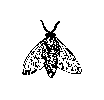
\includegraphics{fly}
\caption{A sample black and white graphic.}
\end{figure}

\begin{figure}
\centering
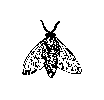
\includegraphics[height=1in, width=1in]{fly}
\caption{A sample black and white graphic
that has been resized with the \texttt{includegraphics} command.}
\end{figure}


As was the case with tables, you may want a figure
that spans two columns.  To do this, and still to
ensure proper ``floating'' placement of tables, use the environment
\textbf{figure*} to enclose the figure and its caption.
and don't forget to end the environment with
{figure*}, not {figure}!

\begin{figure*}
\centering
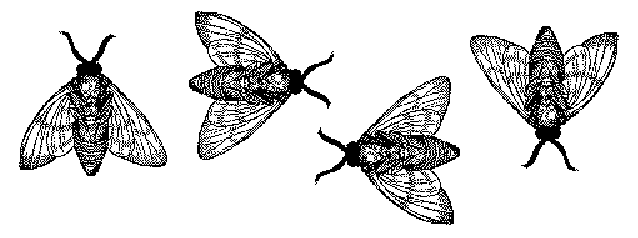
\includegraphics{flies}
\caption{A sample black and white graphic
that needs to span two columns of text.}
\end{figure*}


\begin{figure}
\centering

\includegraphics[height=1in, width=1in]{rosette}
\caption{A sample black and white graphic that has
been resized with the \texttt{includegraphics} command.}
\vskip -6pt
\end{figure}

\subsection{Theorem-like Constructs}
Other common constructs that may occur in your article are
the forms for logical constructs like theorems, axioms,
corollaries and proofs.  There are
two forms, one produced by the
command \texttt{{\char'134}newtheorem} and the
other by the command \texttt{{\char'134}newdef}; perhaps
the clearest and easiest way to distinguish them is
to compare the two in the output of this sample document:

This uses the \textbf{theorem} environment, created by
the\linebreak\texttt{{\char'134}newtheorem} command:
\newtheorem{theorem}{Theorem}
\begin{theorem}
Let $f$ be continuous on $[a,b]$.  If $G$ is
an antiderivative for $f$ on $[a,b]$, then
\begin{displaymath}\int^b_af(t)dt = G(b) - G(a).\end{displaymath}
\end{theorem}

The other uses the \textbf{definition} environment, created
by the \texttt{{\char'134}newdef} command:
\newdef{definition}{Definition}
\begin{definition}
If $z$ is irrational, then by $e^z$ we mean the
unique number which has
logarithm $z$: \begin{displaymath}{\log e^z = z}\end{displaymath}
\end{definition}

Two lists of constructs that use one of these
forms is given in the
\textit{Author's  Guidelines}.
 
There is one other similar construct environment, which is
already set up
for you; i.e. you must \textit{not} use
a \texttt{{\char'134}newdef} command to
create it: the \textbf{proof} environment.  Here
is a example of its use:
\begin{proof}
Suppose on the contrary there exists a real number $L$ such that
\begin{displaymath}
\lim_{x\rightarrow\infty} \frac{f(x)}{g(x)} = L.
\end{displaymath}
Then
\begin{displaymath}
l=\lim_{x\rightarrow c} f(x)
= \lim_{x\rightarrow c}
\left[ g{x} \cdot \frac{f(x)}{g(x)} \right ]
= \lim_{x\rightarrow c} g(x) \cdot \lim_{x\rightarrow c}
\frac{f(x)}{g(x)} = 0\cdot L = 0,
\end{displaymath}
which contradicts our assumption that $l\neq 0$.
\end{proof}

Complete rules about using these environments and using the
two different creation commands are in the
\textit{Author's Guide}; please consult it for more
detailed instructions.  If you need to use another construct,
not listed therein, which you want to have the same
formatting as the Theorem
or the Definition\cite{salas:calculus} shown above,
use the \texttt{{\char'134}newtheorem} or the
\texttt{{\char'134}newdef} command,
respectively, to create it.

\subsection*{A {\secit Caveat} for the \TeX\ Expert}
Because you have just been given permission to
use the \texttt{{\char'134}newdef} command to create a
new form, you might think you can
use \TeX's \texttt{{\char'134}def} to create a
new command: \textit{Please refrain from doing this!}
Remember that your \LaTeX\ source code is primarily intended
to create camera-ready copy, but may be converted
to other forms -- e.g. HTML. If you inadvertently omit
some or all of the \texttt{{\char'134}def}s recompilation will
be, to say the least, problematic.

\section{Conclusions}
This paragraph will end the body of this sample document.
Remember that you might still have Acknowledgments or
Appendices; brief samples of these
follow.  There is still the Bibliography to deal with; and
we will make a disclaimer about that here: with the exception
of the reference to the \LaTeX\ book, the citations in
this paper are to articles which have nothing to
do with the present subject and are used as
examples only.
%\end{document}  % This is where a 'short' article might terminate

%ACKNOWLEDGMENTS are optional
\section{Acknowledgments}
This section is optional; it is a location for you
to acknowledge grants, funding, editing assistance and
what have you.  In the present case, for example, the
authors would like to thank Gerald Murray of ACM for
his help in codifying this \textit{Author's Guide}
and the \textbf{.cls} and \textbf{.tex} files that it describes.

%
% The following two commands are all you need in the
% initial runs of your .tex file to
% produce the bibliography for the citations in your paper.
\bibliographystyle{abbrv}
\bibliography{sigproc}  % sigproc.bib is the name of the Bibliography in this case
% You must have a proper ".bib" file
%  and remember to run:
% latex bibtex latex latex
% to resolve all references
%
% ACM needs 'a single self-contained file'!
%
%APPENDICES are optional
%\balancecolumns
\appendix
%Appendix A
\section{Headings in Appendices}
The rules about hierarchical headings discussed above for
the body of the article are different in the appendices.
In the \textbf{appendix} environment, the command
\textbf{section} is used to
indicate the start of each Appendix, with alphabetic order
designation (i.e. the first is A, the second B, etc.) and
a title (if you include one).  So, if you need
hierarchical structure
\textit{within} an Appendix, start with \textbf{subsection} as the
highest level. Here is an outline of the body of this
document in Appendix-appropriate form:
\subsection{Introduction}
\subsection{The Body of the Paper}
\subsubsection{Type Changes and  Special Characters}
\subsubsection{Math Equations}
\paragraph{Inline (In-text) Equations}
\paragraph{Display Equations}
\subsubsection{Citations}
\subsubsection{Tables}
\subsubsection{Figures}
\subsubsection{Theorem-like Constructs}
\subsubsection*{A Caveat for the \TeX\ Expert}
\subsection{Conclusions}
\subsection{Acknowledgments}
\subsection{Additional Authors}
This section is inserted by \LaTeX; you do not insert it.
You just add the names and information in the
\texttt{{\char'134}additionalauthors} command at the start
of the document.
\subsection{References}
Generated by bibtex from your ~.bib file.  Run latex,
then bibtex, then latex twice (to resolve references)
to create the ~.bbl file.  Insert that ~.bbl file into
the .tex source file and comment out
the command \texttt{{\char'134}thebibliography}.
% This next section command marks the start of
% Appendix B, and does not continue the present hierarchy
\section{More Help for the Hardy}
The sig-alternate.cls file itself is chock-full of succinct
and helpful comments.  If you consider yourself a moderately
experienced to expert user of \LaTeX, you may find reading
it useful but please remember not to change it.
%\balancecolumns % GM June 2007
% That's all folks!
\end{document}
